\chapter{Formal Specification}\label{sec:spec}

\tikzset{%
  every node/.style={
    inner sep=1pt
  },
  every loop/.style={}
}

As we are heading towards implementation considerations in~\cref{sec:impl}, we provide a formal specification of the usage analysis in this section.

Despite being massively more simple than Haskells surface syntax, GHC Core still captures many details inessential to the analysis. 
In order to keep the mathematical formulation as concise as possible, we define the transfer function in terms of a simplified object language in \cref{sec:exp}.

\Cref{sec:dom} introduces the lattice of \emph{usage transformers} the analysis will operate upon. 

Finally, in \cref{sec:transfer} we will see how each syntactic construct of the object language can be denoted by a usage transformer through a \emph{transfer function}.

\section{Object Language}\label{sec:exp}

\begin{figure}[h]
\begin{alignat*}{2}
x,y,z,\sMkPair &\in \sVar \\
e &\in \sExp & {}\Coloneqq{}                    & x \\
  &          & \mathwithin{{}\Coloneqq{}}{\mid} & \sPair{x_1}{x_2} \\
  &          & \mathwithin{{}\Coloneqq{}}{\mid} & \sLam{x}{e} \\
  &          & \mathwithin{{}\Coloneqq{}}{\mid} & \sApp{e}{x} \\
  &          & \mathwithin{{}\Coloneqq{}}{\mid} & \sITE{e_s}{e_t}{e_f} \\
  &          & \mathwithin{{}\Coloneqq{}}{\mid} & \sCase{e_s}{x_1}{x_2}{e_r} \\
  &          & \mathwithin{{}\Coloneqq{}}{\mid} & \sLet{\bind}{e} \\
  &          & \mathwithin{{}\Coloneqq{}}{\mid} & \sLetRec{\binds}{e} \\
\end{alignat*}
\caption{A simple untyped lambda calculus}
\label{fig:exp}
\end{figure}

The formalization of the usage analysis operates on a simple untyped lambda calculus, described in \cref{fig:exp}. 

We extend it in interesting ways to carve out particular details of our analysis.
There are (possibly recursive) \keyword{let} bindings to illustrate sharing of values.
We provide pair constructors, complemented with \keyword{case} expressions to destruct them.
An \keyword{if}/\keyword{then}/\keyword{else} construct will highlight how the analysis will cope with alternative branches of execution.

We draw variable names from an abstract set $\sVar$. 
Of particular note is the identifier $\sMkPair$, which always refers to the pair constructor as a function of two arguments and may not be rebound by a \keyword{let} expression. 
As is customary in both \textcite{card} and \textcite{callarity}, we assume A-normal form \parencite{anf}, so that arguments to applications can only mention identifiers. 
Applications to non-trivial arguments like $\sApp{e_1}{e_2}$ must be rewritten as $\sLet{x_2 = e_2}{\sApp{e_1}{x_2}}$, hence issues concerning sharing only surface while handling \keyword{let}-expressions.

Note that although there are \keyword{if} expressions, we omitted literal syntax to introduce booleans in order to keep the syntax clean. 
Anywhere we write the literals \keyword{True} or \keyword{False}, they desugar to their church encoding $\sLam{t}{\sLam{f}{t}}$ and $\sLam{t}{\sLam{f}{f}}$, respectively.
Our analysis is completely unconcerned by this.

Most code examples will be written in a Haskell-like language anyway, rather than in this object language.
If there are code samples in object language (distinguishable by the typesetting of binders, \eg \hsinl{x} vs. $x$), they should implicitly assumed to be rewritten according to these rules.

\section{Analysis Domain}\label{sec:dom}

The analysis, defined by the transfer function in \cref{sec:transfer}, will denote each syntactic expression with a \emph{usage transformer}. 
This section introduces them from the ground up by defining the relevant concepts.

\subsection{Expression Use and Identifier Usage}

A usage analysis approximates how a use of an expression translates into a use of its subexpressions. Important analysis information includes \parencite{card}:

\begin{enumerate}
\item How many times is the body of a lambda expression evaluated, with respect to its defining scope?
\item How many times is a particular thunk evaluated, with respect to its defining scope?
\item Which components of a syntactic expression are never used, that is, absent?
\end{enumerate}

GHC's Demand analyser integrates a usage analysis that answers these questions by the name of \emph{higher-order cardinality analysis} \parencite{card}. 
Our analysis builds on this approach in that the central lattices have been borrowed unchanged, but have been enriched and distinguished with further semantic meaning.

\begin{figure}
\begin{alignat*}{2}
u   &\in \sUse   &{} \Coloneqq {}& HU \mid U \mid C^n(u) \mid U(u^*_1, u^*_2) \\
u^* &\in \sUsage &{} \Coloneqq {}& A \mid n*u \\
n   &\in \sMulti &{} \Coloneqq {}& 1 \mid \omega
\end{alignat*}
\begin{alignat*}{1}
U(A,A)               &\equiv HU \\
U(\omega*U,\omega*U) &\equiv U \\
C^\omega(U)          &\equiv U
\end{alignat*}
\caption{Syntax of expression $\sUse$ and identifier $\sUsage$ with non-syntactic equalities.}
\label{fig:usg}
\end{figure}

\Cref{fig:usg} depicts the $\sUse$ and the $\sUsage$ lattice. 
Typical for a sharing analysis, $\sMulti$ captures usage multiplicity, of which the only interesting values in our setting are \emph{at most once} ($1$) or \emph{possibly multiple times} ($\omega$).

Semantically, a $\sUse$ describes how the value of an expression is used, after evaluating it to weak head normal form (WHNF) \emph{exactly once}.

\begin{itemize}
\item $U(u^*_1, u^*_2)$ captures the $\sUsage$ of pair components (which we will explain shortly) when the expression evaluates to a pair.
\item $C^n(u)$ suggests that the expression evaluates to a lambda expression. 
      Additionally, the resulting value was called at most $n$ times \emph{relative to the single reduction to WHNF} and the use on the result of each call was not worse than $u$.
\item If the value of an expression wasn't used beyond reduction to WHNF, we can attest the expression a head-use $HU$, the bottom of the lattice. 
      Through the first non-syntactic equality in \cref{fig:usg}, $HU$ is identical to a pair use of $U(A,A)$. 
      This arises naturally when, beyond reduction to the pair constructor, no components of the value were used.
      Other than that, $HU$ can only be unleashed on the first argument of a call to the binary primitive \hsinl{seq}.
      Since \hsinl{seq} can be applied to arguments of any type, expressions of function type can also be head-used.
      When a function expression is in head-use, evaluation will stop immediately after uncovering the outer lambda, the body will not be used.
      This corresponds to a hypothetical ill-typed use $C^0(\uscore)$, meaning the lambda is called 0 times relative to the single reduction of the function expression to WHNF.
\item The most conservative analysis result would be the top of the lattice $U$, representing an unknown use beyond reduction to WHNF.
      Where this differs from head-use is best understood in terms of the attached equalities in \cref{fig:usg}.
      For an expression that evaluates to a pair, unknown use would correspond to the pair use $U(\omega*U,\omega*U)$, e.g.\ the pair components have the worst possible usage.
      A unknown use on a function expression can be interpreted as a use of $C^\omega(U)$ by the last equality: 
      We don't know how the resulting function will be used, so we have to assume multiple calls, each with unknown use. 
\end{itemize}

The syntax for call uses $C^n(u)$ allows to model \emph{multiple} calls of a function expression relative to a \emph{single} reduction to WHNF. 
Yet it is still unclear how expressions can be used in such a way. 
We would need to \emph{share} the work done by reducing the a function expression to WHNF, so that we can call the resulting value at least twice.
Such sharing can be introduced by binding an expression to an identifier. 
By referring to the bound expression through the identifier, we can call the same expression multiple times, while the reduction of the bound expression to WHNF only happens (at most) once. 
Generally, there are various ways to bind an expression to an identifier. 
However, our simple object language was carefully crafted so that sharing is always introduced through \keyword{let} bindings. 
Other binding mechanisms like lambdas and \keyword{case} just alias another binding. 

It is inappropriate to model usage of an identifier with $\sUse$, as identifiers can syntactically occur more than once, or even be absent. 
Yet every use site, or \emph{usage}, unleashes a $\sUse$ on the identifier's bound expression. 
Thus, every identifier has an associated $\sUsage$, that describes how often and how, if at all, the identifier was used.

\begin{itemize}
\item An identifier $\sUsage$ of $A$ represents \emph{absence} of any usage. Right-hand sides of absent bindings are dead code and never used.
\item A $\sUsage$ of $n*u$ represents that the associated identifier was used at most $n$ times, putting its bound expression under combined use $u$.
\end{itemize}

A few examples are instructive in understanding the definitions so far.

\begin{example} 
Consider the following Haskell expression:

\begin{haskellcode}
let a = f 0 
in let b = f 1 
   in case (a, b) of
        (x, y) -> y
\end{haskellcode}

If we put the expression under some use $U$, we find out the following facts by backtracing evaluation:

\begin{itemize}
\item The case binder \hsinl{y} has usage $1*U$, \hsinl{x} is absent ($A$).
\item The usage on case binders translate to a pair use on \hsinl{(a,b)} of $U(A,1*U)$.
\item The pair constructor forwards its component usages to identifier usages for \hsinl{a} ($A$) and \hsinl{b} ($1*U$).
\item Since we recorded a usage of $1*U$ for \hsinl{b}, we put the right-hand side of the binding under use $U$. 
      One call with a single argument results in a usage of $1*C^1(U)$ on \hsinl{f}.
\item We recognize that the binding for \hsinl{a} is dead, so we don't need to look at its right-hand side at all.
\end{itemize}
\end{example}

We just saw a single call usage $1*C^1(U)$ on a free variable \hsinl{f}. 
The following expressions hints at the fact that, in general, right-hand sides of bindings can be put under call uses $C^n_1(C^n_2(\ldots C^n_k(U)\ldots))$ for any $n_i\in\sMulti$.
This is through exploiting currying and sharing through bindings.

\begin{example} 
Consider the multi-call case first:

\begin{haskellcode}
f 0 0 + f 1 1
\end{haskellcode}

This demonstrates how multi-call uses can be introduced. 
A use of $U$ on the expression manifests in two sequential usages $1*C^1(C^1(U))$ of \hsinl{f}, each corresponding so a single call with two arguments. 
These combine to an identifier usage of $\omega*C^\omega(C^1(U))$: 
After all, the lambda expression the function bound to \hsinl{f} reduces to is called twice, resulting in two (non-shared!) values. 
In each case, these function values are immediately called with one argument.

The following snippet illustrates how multi-calls can be shifted further down the chain of call uses:

\begin{haskellcode}
let g = f 0
in g 0 0 + g 1 0
\end{haskellcode}

When this expression is put under use $U$, the subexpression \hsinl{g 1 0 + g 1 0} will expose \hsinl{g} to a usage of $\omega*C^\omega(C^1(U))$, similar to the previous situation.
The expression bound to \hsinl{g} is thus used with $C^\omega(C^1(U))$. Itself being a partial application, the bound right-hand side will subject \hsinl{f} to a usage of $1*C^1(C^\omega(C^1(U)))$.
\end{example}

The $\sUsage$ multiplicity $n*\uscore$ represents how often a given thunk is evaluated. 
Of course, since thunks promise that the bound expression will be reduced to WHNF at most once, after the first evaluation the value will be \emph{memoised} and returned for each subsequent evaluation of the thunk.
As \textcite[Section~2.4]{card} points out, the ritual around memoisation is superfluous if the thunk is not evaluated more than once anyway!
In these cases of \emph{single-entry} thunks, GHC exploits that call-by-need coincides with a leaner call-by-name evaluation strategy.

As the remarks in \textcite[Section~2.5]{card} point out, in a non-strict language with the \hsinl{seq} primitive, it is even possible for functions to be \emph{evaluated} multiple times, yet \emph{called} only once.
If an expression like \hsinl{seq f (f 3)} is put under use $U$, this exposes \hsinl{f} to a usage of $\omega*C^1(U)$: \hsinl{f} is evaluated multiple times, yet called only once.
This is the same argument that \textcite[Appendix~C.2]{warnsbrough} makes with their language of \emph{use} vs. \emph{demand}.

\subsection{Usage signatures}

In the last section we developed vocabulary for describing how an expression is used and to which usage a used expression exposes its free variables. Things don't look so well across function boundaries, though:

\begin{haskellcode}
let f k = 2 * k 5
in let g x = x + 3 
   in f g
\end{haskellcode}

If this is put under the typical use $U$, closer look reveals that \hsinl{k} is used as a continuation inside \hsinl{f}, e.g.\ has the one-shot usage $1*C^1(U)$.
By beta reduction, this is also the usage that \hsinl{f g} exposes \hsinl{g} to.
How do we digest that information in a way that it is available at the call site of \hsinl{f}?

We follow the approach from \textcite{card} and ascribe \emph{usage signatures} to function expressions. Their definition is as follows:
\[
\sigma \in \sSig \Coloneqq \bot \mid \top \mid u^* \to \sigma
\]

Equipped with the right language, we would assign the following usage signatures to \hsinl{f} and \hsinl{g}:

\begin{haskellcode}
f :: ß$1*C^1(U) \to \top$ß
g :: ß$1*U \to \top$ß
\end{haskellcode}

Usage signatures also come with two non-syntactic identities:
\begin{alignat*}{1}
  \omega*U \to \top &\equiv \top \\ 
  A \to \bot        &\equiv \bot
\end{alignat*}

These hint at the fact that usage signatures can be expanded to include arbitrary many arguments (although these are usually prohibited through the type system). 
This is helpful in situations where we only have a usage signature to a call with less arguments available. 

In any case, $\top$ as a usage signature is always a safe conservative approximation. 
The opposite applies to $\bot$, which expands to an infinite sequence of absent usages. 
Where is $\bot$ useful? 
Apart from giving the lattice a least element and thus an identity to the least upper bound operator $\llub$, it arises in error conditions and non-termination. 
Specifically, GHC's primitive \hsinl{raise#} has the usage signature $\omega*U \to \bot$.

Similary, usage signatures elegantly abstract from the myriad of primitive operators in GHC.
For another notworthy example, the \hsinl{seq} operator would have a usage signature of $1*HU \to 1*U \to \top$.

\subsection{Free-variable graph}\label{sec:graph}

\todo{Maybe move this to a prior chapter introducing Call Arity}

Central to GHC's \emph{Call Arity} analysis \parencite{callarity} is an undirected, non-transitive, graph datastructure, representing a called-with relationship between free variables.
Such a co-call graph would contain an edge between two free variables, if it is at all possible that the variables could be evaluated \emph{simultaneously}, in the same evaluation of their containing expression, that is.
Self-edges in co-call graphs correspond to a usage multiplicity of $\omega$, \eg multiple evaluations.

We define co-call graphs as a symmetric binary relation on $\sVar$ and syntax for talking about edges within them:
\[\def\arraystretch{1.5}\arraycolsep=1.4pt
\begin{array}{rcl}
  \gamma \in \sGraph &=& \left\{ \gamma \subseteq \sVar \times \sVar \mid (x,y) \in \gamma \Leftrightarrow (y,x) \in \gamma \right\} \\
  \edge{x_1}{x_2}\in\gamma &\Leftrightarrow& (x_1,x_2) \in \gamma \\
  \neighbors{x}{\gamma} &=& \left\{ y \mid \edge{x}{y} \in \gamma \right\}
\end{array}
\]

We also use the notation $\gamma \setminus_x$ to mean the graph $\gamma$ purged by any edges to $x$.

The cases where co-call graphs yield better results than the usual usage analyses can be boiled down to the following example:

\begin{haskellcode}
let x = expensive 0
in let y = 2*x
   in if b 
      then x 
      else y
\end{haskellcode}

The co-call graph for the \hsinl{if} expression crucially \emph{does not} contain an edge \edge{x}{y}, since usages of both variables can never happen in the same evaluation of the expression.
Knowing that \hsinl{x} is not forced together with \hsinl{y}\footnote{Prior to looking at the right-hand side of \hsinl{y} is, of course.}, we save a self-edge on \hsinl{x} after analysing the right-hand side of \hsinl{y}.

Consequently, \hsinl{x} is recognized of only being evaluated once. 
Other usage analyses like that of GHC's Cardinality Analysis \parencite{card} only model self-loops in the underlying co-call structure (\eg usage multiplicity), so they would fail to recognize the absent edge between \hsinl{x} and \hsinl{y} and conservatively assume \hsinl{x} to be called more than once.

\todo{Mention that this only happens for thunks, or refer to where this is written, \eg \cref{sec:let}}

We enrich the \emph{usage types} of GHC's Cardinality Analysis \parencite{card} with co-call graphs in order to generalise both (c.f. \cref{sec:generalise}).

\subsection{Free-variable use environment}\label{sec:useenv}

Another key ingredient of the analysis domain is an environment in which we track usages of free variables.
While \textcite{card} encode these directly with a mapping from free variables to usages (\emph{multi-demands} in their language), we track usage multiplicity separately in a co-call graph (\cref{sec:graph}).

Thus, we define use environments as partial functions\footnote{Indicated by $\pfun$, following syntax from the Isabelle proof assistant's library ecosystem} with finite domain from free variables $\sVar$ to the $\sUse$ their bound expression is put under:
\[
\varphi \in \sUseEnv = \sVar \pfun \sUse
\]
We write $\dom \varphi$ for the domain of the use environment (or any partial function for that matter).
As with graphs, we also use the notation $\varphi \setminus_x$ to mean $\varphi$ where the domain no longer contains $x$.
Similarly, $\restrict{\varphi}{V}$ is the restriction of $\varphi$ to the domain $V \subseteq \sVar$.

To see how we can recover free-variable $\sUsage$ from a combination of co-call graph and use environment, see \cref{sec:utype}.

\subsection{Usage types and lookup of free-variable usage}\label{sec:utype}

The usage signature mechanism captures all relevant argument usage information for imported global functions.
For local identifiers, there's more relevant information, however.
Consider the following expression:

\begin{haskellcode}
let f x = x + y
in f y
\end{haskellcode}

If put under use $U$, this evaluates \hsinl{y} twice, \eg exposes it to usage $\omega*U$.
That is because \hsinl{y} also has a use site within the function expression bound to \hsinl{f}.

So, in addition to a usage signature, a \emph{usage type} should also include what usage a function exposes its free variables to\footnote{We diverge a little from \textcite{card} here, which define usage types as synonymous to a usage signature.}.
We're quite lucky, just having developed the appropriate structures to capture this!

We define usage types as triples of a co-call graph $\gamma$ (\cref{sec:graph}) and use environment $\varphi$ (\cref{sec:useenv}) for free variables, as well as a usage signature $\sigma$ to capture usage of possible arguments:

\[
\theta \in \sUType \Coloneqq \lTriple{\gamma}{\varphi}{\sigma}
\]

Additionally, with the overloaded notation $\theta \setminus_x$ we mean $\theta$, purged by any mentions of $x$ in its co-call graph and use environment.

As hinted at in \cref{sec:useenv}, we can recover free variable usage in the interplay of co-call graph and use environment, denoted by the following lookup syntax:

\[
\lTriple{\gamma}{\varphi}{\uscore}(x) =
  \begin{cases}
    A, & \text{when } x\notin \dom\varphi \\
    1*\varphi(x), & \text{when } \edge{x}{x} \notin \gamma \\
    \omega*\varphi(x), & \text{otherwise}
  \end{cases}
\]

In our above example, \hsinl{f} has the usage type $\lTriple{\emptyset}{\maplit{y}{U}}{1*U \to \top}$.
Notably, the co-call graph is empty, while the use environment attests \hsinl{y} a use of $U$.
By the rules of usage lookup, this corresponds to usage of $1*U$ exposed on \hsinl{y}.

In fact, a usage type describes how a use on an \emph{expression} translates into usages on arguments and free variables.
So while it is convenient to think of \emph{identifiers} like \hsinl{f} having a usage type, it neglects that work is shared between multiple usages:

\begin{haskellcode}
let x = 5*y
in x + x
\end{haskellcode}

If put under use $U$, this expression exposes \hsinl{x} to usage $\omega*U$. 
The usage type of \hsinl{x} (or, rather its bound expression) exposes \hsinl{y} to usage $1*U$.
This suggests that \hsinl{y} will be exposed to usage $\omega*U$ in the whole expression because of the two uses of \hsinl{x}, which is too conservative:
The binding of \hsinl{x} will share the reduction to WHNF of its right-hand side, exposing \hsinl{y} to a single usage of $1*U$.

We will revisit this when discussing analysis of \keyword{let} bindings.

\subsection{Usage transformers}\label{sec:utrans}

When talking about how an expression uses its free variables, we so far always did presuming a certain use we put the expression under.

To understand why, the following example is instructive:

\begin{haskellcode}
let x = expensive 0
in let y = expensive 1
   in (x, y)
\end{haskellcode}

If put under head use $HU$, this would not expose \hsinl{x} or \hsinl{y} to any usage, thus there are no calls to \hsinl{expensive}.
When put under use $U$ however, both \hsinl{x} and \hsinl{y} are exposed to usage $\omega*U$, in turn calling \hsinl{expensive} twice.
That can make a huge difference in computational work, so it is important to always include the use which an expression is put under.

So, the appropriate way to denote a syntactic expression in terms of usage information is in the form of \emph{usage transformers}\footnote{\textcite{card} define these as \emph{generalised} demand transformers, while their notion of ordinary demand transformers best corresponds to an approximation of our usage transformers}:

\[
\tau \in \sUTrans = \sUse \to \sUType
\]

When denoting expressions, usage transformers map a $\sUse$ the expression is put under to a usage type that describes how the expression uses its arguments and free variables.

Usage transformers of expressions are monotone maps, in line with the intuition that the stronger the use you put an expression under, the stronger is the usage it exposes arguments and free variables to.

\subsection{Lattice Structure}

Previously, we introduced constructs to which we loosely attributed the properties of a lattice. 
This section is dedicated to defining join operators, so that the join-semilattice structure we rely upon in \cref{sec:transfer} is made explicit.
Readers familiar with \textcite{card} may skip this section and \cref{sec:both} after having understood the interplay of co-call graphs and use environment for these operations.

The principal example where joins occur are when combining the analysis results of alternatives of a \keyword{case}-expression. However, since our object language from \cref{sec:exp} only supports very simple \keyword{case}-expressions with the sole purpose of deconstructing pairs, we won't see joins just there. Nevertheless, joins still occur occasionally.

\Cref{fig:lub} shows all definitions of $\llub$ for We start by defining overloaded least upper bound operators $\llub$ for $\sUse$, $\sUsage$ and $\sMulti$

\begin{figure}
\begin{alignat*}{1}
  \Aboxed{u_1 \llub u_2 &= u_3} \\
  U \llub u  &= U \\
  u \llub U  &= U \\
  HU \llub u &= u \\
  u \llub HU &= u \\
  C^{n_1}(u_1) \llub C^{n_2}(u_2) &= C^{n_1 \llub n_2}(u_1 \llub u_2) \\
  U(u^*_1, u^*_2) \llub U(u^*_3, u^*_4) &= U(u^*_1 \llub u^*_3, u^*_2 \llub u^*_4) \\
  &\\
  \Aboxed{u^*_1 \llub u^*_2 &= u^*_3} \\
  A \llub u^* &= u^* \\
  u^* \llub A &= u^* \\ 
  n_1*u^*_1 \llub n_2*u^*_2 &= (n_1 \llub n_2) * (u^*_1 \llub u^*_2) \\
  &\\
  \Aboxed{n_1 \llub n_2 &= n_3} \\
  \omega \llub n &= \omega \\
  n \llub \omega &= \omega \\
  1 \llub 1 &= 1 \\
  &\\
  \Aboxed{\sigma_1 \llub \sigma_2 &= \sigma_3} \\
  \top \llub \sigma &= \top \\
  \sigma \llub \top &= \top \\
  \bot \llub \sigma &= \sigma \\
  \sigma \llub \bot &= \sigma \\
  (u^*_1 \to \sigma_1) \llub (u^*_2 \to \sigma_2) &= u^*_1 \llub u^*_2 \to \sigma_1 \llub \sigma_2 \\
  &\\
  \Aboxed{\gamma_1 \llub \gamma_2 &= \gamma_3} \\
  \gamma_1 \llub \gamma_2 &= \gamma_1 \cup \gamma_2 \\
  &\\
  \Aboxed{\theta_1 \llub \theta_2 &= \theta_3} \\
  \lTriple{\gamma_1}{\varphi_1}{\sigma_1} \llub \lTriple{\gamma_2}{\varphi_2}{\sigma_2} &= \lTriple{\gamma_1 \llub \gamma_2}{\varphi_1 \llub \varphi_2}{\sigma_1 \llub \sigma_2} \\
\end{alignat*}
\label{fig:lub}
\caption{Least upper bound definitions}
\end{figure}

\todo{formulate how $A \pfun B$ is a join semilattice with attached bottom when $B$ is a semijoin lattice. Do I have to be more precise than this?}

We ommitted how $\sUseEnv$, $\sTransEnv$ and $\sUTrans$ are join semilattices for brevity. The first two are partial functions ranging over join semilattices, giving rise to a join semilattice with bottom themselves. For usage transformers the join semilattice structure is the pointwise lattice on $\sUType$. 

Of special interest in \cref{sec:transfer} are \emph{monotone} usage transformers, \eg where a stronger incoming $\sUse$ maps to a stronger resulting $\sUType$, and the approximations thereof.

\subsection{Sequential Composition}\label{sec:both}

Until now, we treated sequential composition rather informally. 
For cases like \hsinl{x + x} it is simple enough to see that \hsinl{x} is exposed to usage $\omega*U$. 
That's less obvious for function calls: For example, the usage \hsinl{f} is exposed to in \hsinl{f 0 0 + f 0 0} is $\omega*C^\omega(C^1(U))$.

How can we formalize the process that combines single usages in such a manner?
The answer to that question bears $\both$ (pronounced 'both') in \cref{fig:both}.

\begin{figure}
\begin{alignat*}{1}
  \Aboxed{u_1 \both u_2 &= u_3} \\
  U \both u  &= U \\
  u \both U  &= U \\
  HU \both u &= u \\
  u \both HU &= u \\
  C^{n_1}(u_1) \both C^{n_2}(u_2) &= C^{\omega}(u_1 \llub u_2) \\
  U(u^*_1, u^*_2) \both U(u^*_3, u^*_4) &= U(u^*_1 \both u^*_3, u^*_2 \both u^*_4) \\
  &\\
  \Aboxed{u^*_1 \both u^*_2 &= u^*_3} \\
  A \both u^* &= u^* \\
  u^* \both A &= u^* \\ 
  n_1*u^*_1 \both n_2*u^*_2 &= \omega * (u^*_1 \both u^*_2) \\
  &\\
  \Aboxed{\varphi_1 \both \varphi_2 &= \varphi_3} \\
  (\varphi_1 \both \varphi_2)\,x &= \begin{cases}
    \varphi_1(x) \both \varphi_2(x),&\text{when } x \in \dom{\varphi_1} \cap \dom{\varphi_2} \\
    \varphi_1(x),&\text{when } x \in \dom{\varphi_1} \\
    \varphi_2(x),&\text{otherwise}
  \end{cases} \\
  &\\
  \Aboxed{\theta_1 \both \theta_2 &= \theta_3} \\
  \lTriple{\gamma_1}{\varphi_1}{\sigma_1} \both \lTriple{\gamma_2}{\varphi_2}{\sigma_2} &= \lTriple{\gamma_1 \llub \gamma_2 \llub (\dom{\varphi_1} \times \dom{\varphi_2})}{\varphi_1 \both \varphi_2}{\sigma_1} \\
\end{alignat*}
\caption{Sequential composition operator $\both$}
\label{fig:both}
\end{figure}

Both calls to \hsinl{f} in \hsinl{f 0 0 + f 0 0}, for example, would result in a usage type of $\lTriple{\emptyset}{\maplit{f}{C^1(C^1(U))}}{\top}$. 
Sequential composition with itself would then yield the expected $\lTriple{\left\{(f,f)\right\}}{\maplit{f}{C^\omega(C^1(U))}}{\top}$.

We also extend the multiplicity notation of usages to usage types to mean exactly this notion of sequential composition with itself:
\begin{alignat*}{1}
  1 * \theta &= \theta \\
  \omega * \theta &= \theta \both \theta
\end{alignat*}

We don't mention usage transformers in \cref{fig:both}, but assume sequential composition on them to be pointwise.

It is worth pointing out that it makes only sense to talk about sequential composition with respect to free variable usage. 

When combining usage types, this means we have to decide which usage signature to return, as combining them has no justifiable meaning. 
We arbitrarily bias the left argument in this regard, which is important to keep in mind for the analysis.

\section{Transfer Function}\label{sec:transfer}

Equipped with the proper language to talk about usage, in this section we associate a denoting usage transformer to a syntactic expression of our object language $\sExp$.

The typical way to do so is via a \emph{transfer function} from expressions to the abstract domain the analysis operates on.
\emph{Abstract interpretation} is the underlying scheme here: We interpret an expression in the approximate semantics of usage transformers.
Usage analysis has also been approached via \emph{type inference} in the past \parencite{warnsbrough}, \parencite{verstoep}.

The following subsections will introduce the different cases of the central transfer function

\[
\transfer{\uscore[x]}{\uscore} \colon \sExp \to \sTransEnv \to \sUTrans
\]

Where $\sTransEnv$ is an environment mapping local \keyword{let} binders to their denoting usage transformer to be unleashed on use sites:

\[
\rho \in \sTransEnv = \sVar \pfun \sUTrans
\]

\subsection{Lambda Abstraction}

Let's start by discussing analysis of lambda expressions:

\[
\transfer{\sLam{x}{e}}{\rho}\,u =
  \begin{cases}
    \lTriple{\emptyset}{\emptymap}{\bot}, & \text{when } u = HU \\
    n*\lTriple{\gamma\setminus_x}{\varphi\setminus_x}{\theta(x) \to \sigma}, & \text{where } 
      \begin{array}{l}
        u \lleq C^n(u_b), \\
        \lTriple{\gamma}{\varphi}{\sigma} = \theta = \transfer{e}{\rho}\,u_b
      \end{array}
  \end{cases}
\]

If the expression is only put under head use, no call happens and there is no need to analyze the lambda body.
Consequently, in that case we can return the $\bot$ element of the $\sUType$ lattice, reflecting no free variable usage and no use of arguments.
Note this only happens in the wild in conjunction with the \hsinl{seq} primitive. 
For example in \hsinl{seq (\\x -> y) 3}, the lambda will be exposed to a head use, while \hsinl{3} will be fully used.

In the other case, we try to approximate the incoming use $u$ by a call use $C^n(u_b)$. 
We'd like that $u$ is some kind of call use, but if you give a programmer enough rope to hang herself (\eg \hsinl{unsafeCoerce}) to bypass the type system, it is possible for $u$ to be incomparable to a call use, \ie $U(1*U)$. 
In this case, the pattern match in the definition would be incomplete.
Thus the slightly less precise, yet still sound notation using $\lleq$: 
In these cases, $u$ always compares to the bottom element $U=C^\omega(U)$.
With some more notation we could have made clear that we want the least upper bound of $u$ that is a call use.

Having figured out $u_b$, the use the body is put under, we can transform this use by analysing the lambda body.
The resulting usage type $\theta=\lTriple{\gamma}{\varphi}{\sigma}$ needs to be post-processed. 
For one, we need to remove the free variable \hsinl{x} from the type, that is captured by lambda binder.
We also need to prepend the usage on the captured identifier to the usage signature which we forward from the body.
At this point, an implementation of the analysis would want to annotate the lambda binder with its usage $\theta(x)$.
Finally, we have to multiply the usage type by the relative body usage $n$.

\subsection{Application and Pairs}\label{sec:app}

The application case $\sApp{e}{x}$ will have to handle the called expression $e$ first to find out the usage signature and then expose $x$ to the argument usage:

\begin{alignat*}{2}
  \transfer{\sApp{e}{x}}{\rho}\,u &=&& \lTriple{\gamma_e}{\varphi_e}{\sigma} \both \liftstar{\transfer{x}{\rho}}\,u^* \\
  &\rlap{ where $\lTriple{\gamma_e}{\varphi_e}{u^* \to \sigma} = \transfer{e}{\rho}\,C^1(u)$} &&\\
\end{alignat*}

For an incoming use $u$ we put $e$ under a single call use of $C^1(u)$. 
In the resulting usage type, we match on the usage signature to get out the argument usage $u^*$ we expose $x$ to.
Since the domain of usage transformers is concerned with expression $\sUse$, we have to provide an function lifting the domain of usage transformers to $\sUsage$s.
This is done by $\liftstar{\uscore}{\uscore}$:

\begin{alignat*}{2}
&\liftstar{\uscore[\tau]}~A &{}={}& \lTriple{\emptyset}{\emptymap}{\bot} \\
&\liftstar{\tau}~(n*u)      &{}={}& n*(\tau~u)
\end{alignat*}

The syntax here is reminiscent of the Kleene star, multiplying the result of $\tau$ by the usage multiplicity. Notably, if $e$ doesn't use its argument, then $u^*=A$ and $x$ will be exposed to no usage at all.

Finally, we sequentially compose the result of using $e$ with the usage type that the lifted usage transformer of $x$ yielded for an exposure to $u^*$. 
After all, both usage types are unleashed in order to satisfy the use on $\sApp e x$.
Note that $\both$ is left-biased with respect to the usage signature.
Therefore the signature of the whole application expression is that of $e$, relieved by the usage of $x$. 

The seemingly unrelated case of pair literals is handled by the same application mechanism:

\[
\transfer{\sPair{x_1}{x_2}}{\rho} = \transfer{\sApp{\sApp{\sMkPair}{x_1}}{x_2}}{\rho}
\]

Representative for any product type, we handle pairs as applications to a special identifier for the pair constructor, $\sMkPair$.
As mentioned in \cref{sec:exp}, $\sMkPair$ is special in that it cannot be rebound (\eg shadowed) by \keyword{let} bindings.

Although desugaring pairs in such a way is a nice way to keep the definition short, it is worth pointing out that the complexity is just delegated to the usage transformer for the $\sMkPair$ identifier, which will have to provide an appropriate usage signature. 
We will handle this in the variable case.

\subsection{Case Expression}

The limited \keyword{case}-expressions of our object language serve the sole purpose of desctructuring pairs.

We denote it with a usage transformer that makes it evident that we are dealing with a \emph{backwards analysis}:

\begin{alignat*}{2}
  \transfer{\sCase{e_s}{x}{y}{e_r}}{\rho}\,u &{}={}&& \theta_r\setminus_{x,y} \both \transfer{e_s}{\rho}\,U(\theta_r(x),\theta_r(y)) \\
   \text{where} \\
   \theta_r &{}={}&& \transfer{e_r}{\rho}\,u 
\end{alignat*}

Observe from the flow of information that in order to analyze the scrutinee $e_s$, we first have to analyze the (in general:\ every) case branch $e_r$. 
Case statements are Haskell's basic construct to specify evaluation order: 
A typical operational semantics would first analyze the scrutinee, then choose the appropriate case branch.

The denoting usage transformer will apply the incoming use to the case branch.
In the resulting usage type $\theta_r$ we can look up the usage the product component binders $x$ and $y$ are exposed to.
Based on that, we can formulate the use on the scrutinee as $U(\theta_r(x), \theta_r(y))$.

Finally, we sequentially compose the usage type of the case alternative (purged of the case binders) with the usage type of the scrutinee under the calculated use.
The left argument to $\both$ is $\theta_r$ since the resulting usage signature should be that of the case alternative, rather than that of the scrutinee.

\subsection{\keyword{if} Expressions}

In a more elaborate core language like that of GHC, there would be a single \keyword{case} expression handling algebraic data types with any number of cases.

However, to keep the transfer function simple and concerns orthogonal, it is favorable to separate out \keyword{case} statements with multiple branches into an \keyword{if}/\keyword{then}/\keyword{else} construct.

\begin{alignat*}{2}
  \transfer{\sITE{e_s}{e_t}{e_f}}{\rho}\,u &{}={}&& (\transfer{e_t}{\rho}\,u \llub \transfer{e_f}{\rho}\,u) \both \transfer{e_s}{\rho} U \\
\end{alignat*}

This looks like a simpler version of the transfer function on \keyword{case} expressions.
Yet the usage type of \keyword{then} and \keyword{else} branches are joined together before sequentially combining with the usage type of the scrutinee.
For a general \keyword{case} expression, we would join analysis results of all branches together in much the same way.

We primarily need \keyword{if} expressions to introduce missing edges in a co-call graph, for the sake of illustrative examples. 
For instance, in the object language expression $\sITE{b}{t}{f}$ there will be no edge $\edge{t}{f}$ in the co-call graph.

\subsection{Variables}\label{sec:var}

For the variable case, we want the following things to happen:

\begin{itemize}
\item Note the single evaluation of $x$. We need this information for annotating identifiers, as well as analysing bound expressions later on.
\item For any free variables, track to what usage the use on $x$ exposes them to. This is important for \keyword{let}-bound identifiers.
\item Tack a proper usage signature onto the usage type in the case of call uses.
\end{itemize}

We begin with an auxiliary transformer that captures the first point. 
This is the definition for $\tau^1_x$, the transformer putting the variable $x$ once under the incoming use $u$:

\[
\tau^1_x~u = \lTriple{\emptyset}{\maplit{x}{u}}{\top}
\]

Co-call graph and use environment convey that $x$ is exposed to usage $1*u$, while $\top$ is always a sound approximation to argument usage without knowing more about $x$.

With that in mind, we can have a look at the transfer function for variables:

\[
\transfer{x}{\rho} =
  \begin{cases}
    \tau_{\sMkPair}, & \text{when } x = \sMkPair \\
    \rho(x) \both \tau^1_x, & \text{when } x\in \dom{\rho} \\
    \tau^1_x, & \text{otherwise}
  \end{cases}
\]

Ignoring the first two cases for a moment, the default case denotes the single use of $x$ with $\tau^1_x$.

However for \keyword{let}-bound identifiers, which are handled by the second case, we can do better than that. 

For every \keyword{let} binder, we have a usage transformer denoting its bound expression available in $\rho$.
The (potential) call to $x$ is approximated by unleashing that usage transformer at the call site.
This is analogous to the \letdnsc{} rule in \textcite{card} and comes with the same trade-off, discussed in \cref{sec:let}.
We still have to remember the call to $x$ and do so by sequentially composing with $\tau^1_x$.
Recall that the sequential composition operator $\both$ is left-biased with respect to the usage signature, so the result will have the signature of $\rho(x)$ instead of $\top$.

The remaining first case handles calls to the pair constructor $\sMkPair$ by delegating to another auxiliary usage transformer $\tau_{\sMkPair}$:

\[
\tau_{\sMkPair}~u =
  \begin{cases}
    \lTriple{\emptyset}{\emptymap}{\bot}, & \text{when } u \lless C^1(C^1(\uscore)) \\
    \lTriple{\emptyset}{\emptymap}{u^*_1 \to u^*_2 \to \top}, & \text{when } u = C^1(C^1(U(u^*_1,u^*_2))) \\
    \lTriple{\emptyset}{\emptymap}{\top}, & \text{otherwise}
  \end{cases}
\]

As mentioned in \cref{sec:app}, we desugar pair literals as binary applications to the pair constructor $\sMkPair$.

Information on free variable usage is uninteresting for constructors, in contrast to their usage signatures.

When the incoming use is less than $C^1(C^1(U))$ (\eg $C^1(HU)$), we are dealing with a partial constructor application. 
In that case, the components of the pair are unused and we propagate back a usage signature of $\bot$.

For the second case it is illustrative to consider an application to the pair constructor like $\sApp{\sApp{\sMkPair}{x}}{y}$.

If put under use $U(1*U, A)$, we want the component usages to propagate to $x$ and $y$ through a usage signature announced by $\sMkPair$.
What is the use that $\sMkPair$ is put under? 
The use on the whole application, wrapped in two single shot calls, $C^1(C^1(U(1*U, A))$.
For this specific incoming use, we want the transformer denoting $\sMkPair$ to have a usage signature of $1*U \to A \to \bot$.
In general, for saturated single calls with arity at least as high as the data constructor's (that of pairs is two), we can propagate the usage of the pair components in the usage signature.

The last case handles all other incoming uses with a conservative usage signature of $\top$.

\subsection{Non-recursive Let}\label{sec:let}

Resolution of \keyword{let} bindings often bears interesting design decisions of an analysis.

This analysis is no exception to that rule:
It combines the ideas from co-call graphs \parencite{callarity} with the general approach of \textcite{card}.

As pointed out in \textcite[section~3.5]{card}, on one hand, we want to unleash calls right at their use site, as if it were inlined, to have a usage signature available:

\begin{haskellcode}
  let b t f = t
  in b 0 (expensive 0)
\end{haskellcode}

The usage signature for \hsinl{b} would reveal that the \hsinl{expensive} computation is never needed.
Thus, we ideally want to analyse \keyword{let} bindings in a \emph{downward} manner, analyzing bound expressions before \keyword{let}-bodies.
In \textcite{card} this is accounted for by the \letdnsc{} rule.

As they suggest in section~3.6 and we alluded to in \cref{sec:utype} however, this approach loses the shared work of bringing the bound expression to WHNF:

\begin{haskellcode}
let x = 5*y
in x + x
\end{haskellcode}

Unleashing the usage type of \hsinl{x} at each use site would cause the analysis to report \hsinl{y} to be exposed to usage $\omega*U$, where in reality evaluation of the right hand side of \hsinl{x} is shared, hence \hsinl{y} is only exposed to usage $1*U$.

In these cases analysis should proceed in an \emph{upward} manner: 
Knowing that the \keyword{let}-body exposes \hsinl{x} to usage $\omega*U$, we can analyze the bound expression once in use $U$. 
Remarkably, this means just one evalution to WHNF, exposing \hsinl{y} to usage $1*U$.

This is embodied in the \letupsc{} rule of \textcite{card}.

At the point where upward analysis unleashes usage types of the bound expression, precise co-call information is no longer available.
As discussed in \cref{sec:graph}, that is why co-call graphs are valuable. Recall the example from \cref{sec:graph}:

\begin{haskellcode}
let x = expensive 0
in let y = 2*x
   in if b 
      then x 
      else y
\end{haskellcode}

The \letupsc{} rule would assign \hsinl{x} a usage of $\omega*U$. 
A co-call graph captures the mutual exclusive call relationship between \hsinl{x} and \hsinl{y}, so evaluation of \hsinl{y} does not need to be sequentially composed with the other usage of \hsinl{x}, resulting in \hsinl{x} being exposed to the expected usage $1*U$.

Note that the \letdnsc{} approach would not suffer from this imprecision: 
If the usage type of \hsinl{x}'s bound expression's evaluation was immediately unleashed at its use sites, usages would be on different branches and analysis results would be fine.

As a result, analysis of thunks (\eg bindings which are not in WHNF) should respect sharing in a similar way to \letupsc{}, while function calls should be treated in \letdnsc{}-style, as if calls where inlined.
Therefore, we flavor the approach of \textcite{card} with co-call graphs from \textcite{callarity} to mitigate the discussed imprecision of \letupsc{}.

That said, here is the transfer function on non-recursive \keyword{let} bindings:
\begin{alignat*}{2}
  \transfer{\sLet{\bind}{e}}{\rho}\,u &{}={}&& (\cmblet{\theta}{\maplit{x_1}{\theta_1}}) \setminus_{x_i} \\
  \text{where} \\
   \tau_1 &{}={}&& \transfer{e_1}{\rho} \\
   \rho' &{}={}&& \maplit{x_1}{\letdown{\tau_1}{e_1}}\rho \\ 
   \theta &{}={}&& \transfer{e}{\rho'}\,u \\ 
   \theta_1 &{}={}&& \liftqm{\letup{\tau_1}{e_1}}{\theta(x_1)}
\end{alignat*}

Let us start by understanding the auxiliary definitions. 

The usage transformer $\tau_1$ is the denotation of the bound expression $e_1$. 
We add this new usage transformer to the transformer environment $\rho$ under the identifier $x_1$, yielding a new environment $\rho'$ which we need to analyse $e$.

There is a small catch though: Actually we don't extend $\rho$ with $\tau_1$ directly, but a version modified by the \letdnsc{} operator $\letdown{\uscore}{\uscore} \colon \sUTrans \to \sExp \to \sUTrans$, which we define shortly.
This makes sense: The way the transformers in $\rho$ are unleashed in the variable case (\cf \cref{sec:var}) corresponds to the \letdnsc{} rule in \textcite{card}.

Equipped with the extended transformer environment $\rho'$, we can proceed to analyse the body $e$. 
We put its denotation under the incoming use $u$ and observe a usage type $\theta$.

\todo{Mention where an implementation would annotate stuff and that we would update the syntax tree with the final \letupsc{} run over the bound expression}

This usage type has information about which usage $x_1$ was exposed to in the body, expressed as $\theta(x_1)$. 
Broadly speaking, $\theta_1$ is the result of putting the bound expression, denoted by $\tau_1$, under this usage for a \letupsc{}-like treatment.

For this, $\tau_1$ is again modified, this time by the \letupsc{} operator $\letup{\uscore}{\uscore} \colon \sUTrans \to \sExp \to \sUTrans$.

The resulting usage transformer is then lifted to the domain of $\sUsage$s with $\liftqm{\uscore}{\uscore}$. 
We already saw a similar operator, $\liftstar{\uscore}{\uscore}$ in \cref{sec:app}. 
This one lifts with a question mark, reminiscent of `zero or one times'.
\begin{alignat*}{2}
&\liftqm{\uscore[\tau]}~A     &{}={}& \lTriple{\emptyset}{\emptymap}{\bot} \\
&\liftqm{\tau}~(\uscore[n]*u) &{}={}& \tau~u
\end{alignat*}

Now is a good time to introduce the \letdnsc{} and \letupsc{} operators:
\begin{alignat*}{1}
&\zap~{}\colon\sUType \to \sUType \\
&\zap~\lTriple{\uscore}{\uscore}{\sigma} = \lTriple{\emptyset}{\emptymap}{\sigma}
\end{alignat*}
\begin{alignat*}{2}
  &\letup{\uscore[\tau]}{\uscore[e]} &\mathmakesamewidth[c]{{}=}{\colon} &\sUTrans \to \sExp \to \sUTrans \\
  &\letup{\tau}{e} &{}={}&
  \begin{cases}
    \zap\circ\tau, & \text{when } e \text{ is in WHNF} \\
    \tau, & \text{otherwise}
  \end{cases} \\
\\
  &\letdown{\uscore[\tau]}{\uscore[e]} &\mathmakesamewidth[c]{{}=}{\colon} &\sUTrans \to \sExp \to \sUTrans \\
  &\letdown{\tau}{e} &{}={}&
  \begin{cases}
    \zap, & \text{when } e \text{ is in WHNF} \\
    \zap\circ\tau, & \text{otherwise}
  \end{cases}
\end{alignat*}

The $\zap$ function deletes any information about free variables from a usage type.
The \letdnsc{} operator $\zap$s free variable information exactly when the \letupsc{} operator does not, so we can be sure that for every \keyword{let}-bound identifier, we either unleash free variable information in \letupsc{} or \letdnsc{} fashion, but never both.

When do we unleash \letupsc{}-style? For those identifiers whose bound expression $e$ is not a value. 
Conversely, if the bound expression $e$ is already a value, usage information on free variables will be unleashed at use sites, \letdnsc{}-style.

With the ancillary definitions explained, we visit the final expression defining the denoting transformer.
The expression $\cmblet{\theta}{\maplit{x_1}{\theta_1}}$ sequentially composes $\theta$ with $\theta_1$. 
However it relates only a subset of the free variables of $\theta$ to those of $\theta_1$ with co-call edges.
This composition step is critical to the precision of Call Arity \parencite{callarity}, where resolution with co-call graphs is first described.
Only the neighbors of $x_1$ in $\theta$ can be co-called with everything from $\theta_1$, other co-call edges are ommitted.
The $\cmblet{\uscore}{\uscore}$ operator can be thought of as a substitution operator for variable graphs.
In $\cmblet{\theta}{\maplit{x_1}{\theta_1}}$, the operator will substitute every mention of $x_1$ by its associated usage type $\theta_1$ and inherit all relevant co-call edges in the process.

We see in a minute an example that clears things up, but let us first have a look at the definition of this substitution operator:
\begin{alignat*}{2}
  \cmblet{\uscore[\theta]}{\mathmakesamewidth[l]{\maplit{x_i}{\lTriple{\gamma_i}{\varphi_i}{\uscore}}\mu}{\uscore[\emptymap]}} &\mathmakesamewidth[c]{~~=}\colon &&\sUType \to (\sVar \pfun \sUType) \to \sUType \\
  \cmblet{\theta}{\mathmakesamewidth[l]{\maplit{x_i}{\lTriple{\gamma_i}{\varphi_i}{\uscore}}\mu}{\emptymap}} &{}={}&& \theta \\
  \cmblet{\theta}{\maplit{x_i}{\lTriple{\gamma_i}{\varphi_i}{\uscore}}\mu} &{}={}&& \lTriple{\gamma}{\varphi}{\sigma} \\
  \text{where} \\ 
    \lTriple{\gamma'}{\varphi'}{\sigma} &{}={}&& \cmblet{\theta}{\mu} \\ 
    N &{}={}&& \neighbors{x_i}{\gamma'} \\
    \gamma &{}={}&& \gamma' \llub \gamma_i \llub (N \times \dom{\varphi_i}) \\
    \varphi &{}={}&& \varphi' \llub \varphi_i \llub (\restrict{\varphi'}{N}\both \varphi_i)
\end{alignat*}

\todo{Think about formatting this better}

Apart from recursing over the entire finite map in the second parameter (which makes it a well-defined function), it works very much like the sequential composition operator $\both$ on usage types from \cref{sec:both}.

The only thing in which this substitution operator is more precise is in selecting only a subset $N$ of variables from $\dom{\varphi'}$ which to sequentially compose with $\dom{\varphi_i}$.

As \textcite{callarity} proves, it is safe to choose only the neighbors of $x_i$ in the co-call graph for this:
All other variables are not actually evaluated together with $x_i$, so we should not need to sequentially compose them.

Mind that the substitution operator will not actually delete $x_i$ from the usage type, so the transfer function must do so after substitution.
The reason for this is anticipation of recursive binding groups, where the fixed-point iteration relies on binder usage from the last iteration.

The substitution operator is strongly related to \emph{composition graphs} $G_0[G_1,\ldots,G_n]$ as introduced in \textcite[pp.~109]{agt}, where the $n$ vertices in the \emph{outer factor} $G_0$ are substituted by the \emph{inner factors} $G_1,\ldots,G_n$. 

\begin{example}
  Consider the following non-closed Haskell expression:
  \begin{haskellcode}
    let x = 5*a + 3*b
    in if z
       then x
       else y
  \end{haskellcode}

  We focus on how the \keyword{let} binding will be resolved. For the sake of the example we can assume that all mentioned identifiers have bound non-function expressions which are not in WHNF, thus usage types are unleashed \letupsc{} style.

  For an incoming use of $U$, all particular uses in this example are $U$ and all usage signatures are $\top$.
  Only the co-call graphs are interesting.

  Analysis of the \keyword{if} expressions yields the usage type $\theta$. 
  It reveals that \hsinl{x} is exposed to usage $1*U$, so its bound expression is put under use $U$.
  This results in a usage type $\theta_1$ for the bound expression.
  The associated co-call graphs $\gamma$ and $\gamma_1$ are the following:
  \begin{align*}
    \gamma &= 
    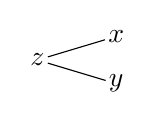
\begin{tikzpicture}[baseline={(0.base)}]
      \node (0) {$z$};
      \node at (1,0.3) (1) {$x$};
      \node at (1,-0.3) (2) {$y$};
      \draw (0) -- (1);
      \draw (0) -- (2);
    \end{tikzpicture}
    &
    \gamma_1 =&
    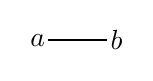
\begin{tikzpicture}[baseline={(0.base)}]
      \node (0) {$a$};
      \node (1) at (1,0) {$b$};
      \draw (0) -- (1);
    \end{tikzpicture}
  \end{align*}

  The substitution step will substitute $\gamma_1$ into $x$ and immediately flatten the resulting hypergraph:
  \begin{align*}
    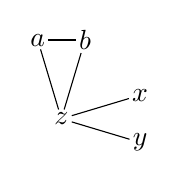
\begin{tikzpicture}[baseline={(0.base)}]
      \node (0) {$z$};
      \node at (1,0.3) (1) {$x$};
      \node at (1,-0.3) (2) {$y$};
      \node at (-0.3, 1) (3) {$a$};
      \node at (0.3, 1) (4) {$b$};
      \draw (3) -- (4);
      \draw (0) -- (1);
      \draw (0) -- (3);
      \draw (0) -- (4);
      \draw (0) -- (2);
    \end{tikzpicture}
  \end{align*}

  Finally, the transfer function will delete all mentions of $x$ from the usage type, resulting in the final co-call graph
  \begin{align*}
    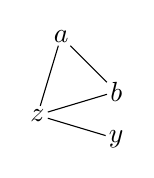
\begin{tikzpicture}[baseline={(0.base)}]
      \node (0) {$z$};
      \node at (1,-0.3) (2) {$y$};
      \node at (0.3, 1) (3) {$a$};
      \node at (1, 0.3) (4) {$b$};
      \draw (3) -- (4);
      \draw (0) -- (3);
      \draw (0) -- (4);
      \draw (0) -- (2);
    \end{tikzpicture}
  \end{align*}

  Note that \hsinl{a} and \hsinl{b} are not co-called with \hsinl{y}, as expected.
\end{example}

\begin{example}
  For another example that focuses on the \letdnsc{} rule instead of the \letupsc{} rule, consider the following slightly modified variant from a moment ago:
  \begin{haskellcode}
    let f x = 5*a + 3*b
    in if z
       then f y
       else y
  \end{haskellcode}

  This is the nearly same example as before, only the work of the bound expression is now hidden behind a lambda. 
  So the expression is in WHNF and \hsinl{f} will be unleashed according to \letdnsc{}.

  When analysing that \keyword{let} binding, we extend the transformer environment with the usage transformer $\tau_1$, denoting the expression bound to \hsinl{f}, to yield $\rho'$.
  
  Analysis proceeds with the \keyword{let} body. The call site of \hsinl{f} entails a lookup in $\rho'$ and will unleash the usage type (\cf the variable case in \cref{sec:var})
  \begin{align*}
    \rho'(f)\,C^1(U) \both \tau^1_f\,C^1(U) &=
    \lTriple{
      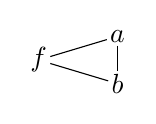
\begin{tikzpicture}[baseline={(0.base)}]
        \node (0) {$f$};
        \node at (1,0.3) (1) {$a$};
        \node at (1,-0.3) (2) {$b$};
        \draw (0) -- (1);
        \draw (0) -- (2);
        \draw (1) -- (2);
      \end{tikzpicture}
    }{\left[f \mapsto C^1(U), a \mapsto U, b \mapsto U\right]}{A \to \top}
  \end{align*}
  
  The usage signature conveys that \hsinl{f} does not use its argument, so the call does not use \hsinl{y} at all.

  That means the whole \hsinl{if} expression will have the co-call graph
  \begin{align*}
      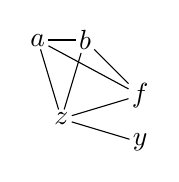
\begin{tikzpicture}[baseline={(0.base)}]
        \node (0) {$z$};
        \node at (1,0.3) (1) {$f$};
        \node at (1,-0.3) (2) {$y$};
        \node at (-0.3, 1) (3) {$a$};
        \node at (0.3, 1) (4) {$b$};
        \draw (3) -- (4);
        \draw (0) -- (1);
        \draw (0) -- (3);
        \draw (0) -- (4);
        \draw (0) -- (2);
        \draw (1) -- (3);
        \draw (1) -- (4);
      \end{tikzpicture}
  \end{align*}

  This differs from the prior example's graph only in that there are co-call edges between \hsinl{f} and the free variables of its bound expression.
  These are irrelevant, however, as for non-recursive \keyword{let} these can never introduce loops on \hsinl{f}. 
  After all, how would \hsinl{f}'s bound expression call itself? 

  The final co-call graph after deleting \hsinl{f} is exactly the same as in the preceding example:
  \begin{align*}
    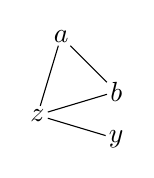
\begin{tikzpicture}[baseline={(0.base)}]
      \node (0) {$z$};
      \node at (1,-0.3) (2) {$y$};
      \node at (0.3, 1) (3) {$a$};
      \node at (1, 0.3) (4) {$b$};
      \draw (3) -- (4);
      \draw (0) -- (3);
      \draw (0) -- (4);
      \draw (0) -- (2);
    \end{tikzpicture}
  \end{align*}

  This exemplifies that in the case of functions, \letdnsc{} is as precise as \letupsc{} with co-call graphs.
\end{example}


\subsection{Recursive Let}\label{sec:letrec}

\begin{alignat*}{2}
&\transfer{\sLet{\binds}{e}}{\rho}\,u &{}={}& \cmblet{\theta}{\maplit[\overline]{x_i}{\theta_i}} \\
   &&&\text{where }
     \overline{\tau_i = \transfer{e_i}{\rho'}},~
     \rho' = \maplit[\overline]{x_i}{\letdown{\tau_i}{x_i}}\rho,~
     \theta = \transfer{e}{\rho}\,u \llub \transfer{\sLet{\binds}{e}}{\rho}\,u,~
     \overline{\theta_i = \liftqm{\letup{\transfer{e_i}{\rho'}}{x_i}}\,(\theta(x_i) \both \theta(x_i))}
\end{alignat*}
